% Created by tikzDevice version 0.10.1 on 2016-09-01 14:52:48
% !TEX encoding = UTF-8 Unicode
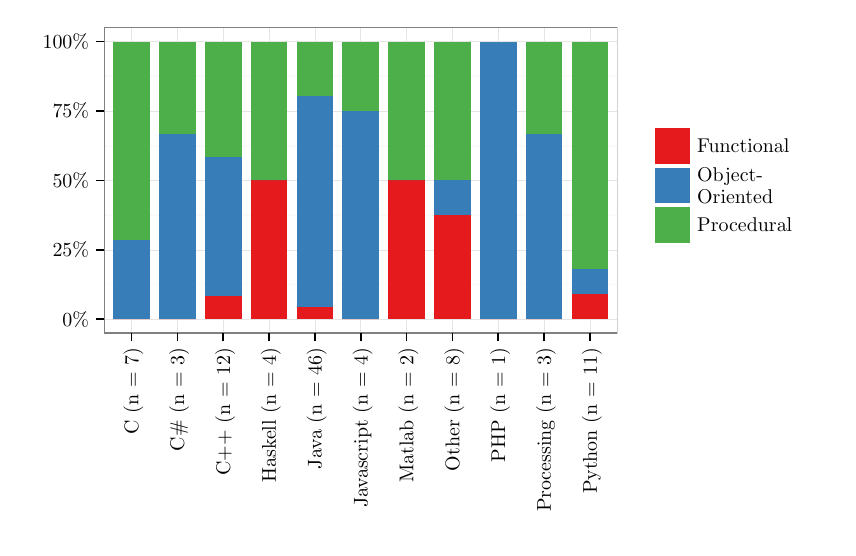
\begin{tikzpicture}[x=1pt,y=1pt]
\definecolor{fillColor}{RGB}{255,255,255}
\path[use as bounding box,fill=fillColor,fill opacity=0.00] (0,0) rectangle (289.08,180.67);
\begin{scope}
\path[clip] (  0.00,  0.00) rectangle (289.08,180.67);
\definecolor{drawColor}{RGB}{255,255,255}
\definecolor{fillColor}{RGB}{255,255,255}

\path[draw=drawColor,line width= 0.6pt,line join=round,line cap=round,fill=fillColor] (  0.00,  0.00) rectangle (289.08,180.67);
\end{scope}
\begin{scope}
\path[clip] ( 27.58, 70.28) rectangle (213.11,180.67);
\definecolor{fillColor}{RGB}{255,255,255}

\path[fill=fillColor] ( 27.58, 70.28) rectangle (213.11,180.67);
\definecolor{drawColor}{gray}{0.98}

\path[draw=drawColor,line width= 0.6pt,line join=round] ( 27.58, 87.84) --
	(213.11, 87.84);

\path[draw=drawColor,line width= 0.6pt,line join=round] ( 27.58,112.93) --
	(213.11,112.93);

\path[draw=drawColor,line width= 0.6pt,line join=round] ( 27.58,138.02) --
	(213.11,138.02);

\path[draw=drawColor,line width= 0.6pt,line join=round] ( 27.58,163.11) --
	(213.11,163.11);
\definecolor{drawColor}{gray}{0.90}

\path[draw=drawColor,line width= 0.2pt,line join=round] ( 27.58, 75.29) --
	(213.11, 75.29);

\path[draw=drawColor,line width= 0.2pt,line join=round] ( 27.58,100.38) --
	(213.11,100.38);

\path[draw=drawColor,line width= 0.2pt,line join=round] ( 27.58,125.48) --
	(213.11,125.48);

\path[draw=drawColor,line width= 0.2pt,line join=round] ( 27.58,150.57) --
	(213.11,150.57);

\path[draw=drawColor,line width= 0.2pt,line join=round] ( 27.58,175.66) --
	(213.11,175.66);

\path[draw=drawColor,line width= 0.2pt,line join=round] ( 37.52, 70.28) --
	( 37.52,180.67);

\path[draw=drawColor,line width= 0.2pt,line join=round] ( 54.08, 70.28) --
	( 54.08,180.67);

\path[draw=drawColor,line width= 0.2pt,line join=round] ( 70.65, 70.28) --
	( 70.65,180.67);

\path[draw=drawColor,line width= 0.2pt,line join=round] ( 87.21, 70.28) --
	( 87.21,180.67);

\path[draw=drawColor,line width= 0.2pt,line join=round] (103.78, 70.28) --
	(103.78,180.67);

\path[draw=drawColor,line width= 0.2pt,line join=round] (120.34, 70.28) --
	(120.34,180.67);

\path[draw=drawColor,line width= 0.2pt,line join=round] (136.91, 70.28) --
	(136.91,180.67);

\path[draw=drawColor,line width= 0.2pt,line join=round] (153.47, 70.28) --
	(153.47,180.67);

\path[draw=drawColor,line width= 0.2pt,line join=round] (170.04, 70.28) --
	(170.04,180.67);

\path[draw=drawColor,line width= 0.2pt,line join=round] (186.60, 70.28) --
	(186.60,180.67);

\path[draw=drawColor,line width= 0.2pt,line join=round] (203.17, 70.28) --
	(203.17,180.67);
\definecolor{fillColor}{RGB}{228,26,28}

\path[fill=fillColor] ( 30.89, 75.29) rectangle ( 44.14, 75.29);
\definecolor{fillColor}{RGB}{55,126,184}

\path[fill=fillColor] ( 30.89, 75.29) rectangle ( 44.14,103.97);
\definecolor{fillColor}{RGB}{77,175,74}

\path[fill=fillColor] ( 30.89,103.97) rectangle ( 44.14,175.66);
\definecolor{fillColor}{RGB}{228,26,28}

\path[fill=fillColor] ( 47.46, 75.29) rectangle ( 60.71, 75.29);
\definecolor{fillColor}{RGB}{55,126,184}

\path[fill=fillColor] ( 47.46, 75.29) rectangle ( 60.71,142.20);
\definecolor{fillColor}{RGB}{77,175,74}

\path[fill=fillColor] ( 47.46,142.20) rectangle ( 60.71,175.66);
\definecolor{fillColor}{RGB}{228,26,28}

\path[fill=fillColor] ( 64.02, 75.29) rectangle ( 77.27, 83.66);
\definecolor{fillColor}{RGB}{55,126,184}

\path[fill=fillColor] ( 64.02, 83.66) rectangle ( 77.27,133.84);
\definecolor{fillColor}{RGB}{77,175,74}

\path[fill=fillColor] ( 64.02,133.84) rectangle ( 77.27,175.66);
\definecolor{fillColor}{RGB}{228,26,28}

\path[fill=fillColor] ( 80.59, 75.29) rectangle ( 93.84,125.48);
\definecolor{fillColor}{RGB}{55,126,184}

\path[fill=fillColor] ( 80.59,125.48) rectangle ( 93.84,125.48);
\definecolor{fillColor}{RGB}{77,175,74}

\path[fill=fillColor] ( 80.59,125.48) rectangle ( 93.84,175.66);
\definecolor{fillColor}{RGB}{228,26,28}

\path[fill=fillColor] ( 97.15, 75.29) rectangle (110.40, 79.66);
\definecolor{fillColor}{RGB}{55,126,184}

\path[fill=fillColor] ( 97.15, 79.66) rectangle (110.40,156.02);
\definecolor{fillColor}{RGB}{77,175,74}

\path[fill=fillColor] ( 97.15,156.02) rectangle (110.40,175.66);
\definecolor{fillColor}{RGB}{228,26,28}

\path[fill=fillColor] (113.72, 75.29) rectangle (126.97, 75.29);
\definecolor{fillColor}{RGB}{55,126,184}

\path[fill=fillColor] (113.72, 75.29) rectangle (126.97,150.57);
\definecolor{fillColor}{RGB}{77,175,74}

\path[fill=fillColor] (113.72,150.57) rectangle (126.97,175.66);
\definecolor{fillColor}{RGB}{228,26,28}

\path[fill=fillColor] (130.28, 75.29) rectangle (143.53,125.48);
\definecolor{fillColor}{RGB}{55,126,184}

\path[fill=fillColor] (130.28,125.48) rectangle (143.53,125.48);
\definecolor{fillColor}{RGB}{77,175,74}

\path[fill=fillColor] (130.28,125.48) rectangle (143.53,175.66);
\definecolor{fillColor}{RGB}{228,26,28}

\path[fill=fillColor] (146.85, 75.29) rectangle (160.10,112.93);
\definecolor{fillColor}{RGB}{55,126,184}

\path[fill=fillColor] (146.85,112.93) rectangle (160.10,125.48);
\definecolor{fillColor}{RGB}{77,175,74}

\path[fill=fillColor] (146.85,125.48) rectangle (160.10,175.66);
\definecolor{fillColor}{RGB}{228,26,28}

\path[fill=fillColor] (163.41, 75.29) rectangle (176.66, 75.29);
\definecolor{fillColor}{RGB}{55,126,184}

\path[fill=fillColor] (163.41, 75.29) rectangle (176.66,175.66);
\definecolor{fillColor}{RGB}{77,175,74}

\path[fill=fillColor] (163.41,175.66) rectangle (176.66,175.66);
\definecolor{fillColor}{RGB}{228,26,28}

\path[fill=fillColor] (179.98, 75.29) rectangle (193.23, 75.29);
\definecolor{fillColor}{RGB}{55,126,184}

\path[fill=fillColor] (179.98, 75.29) rectangle (193.23,142.20);
\definecolor{fillColor}{RGB}{77,175,74}

\path[fill=fillColor] (179.98,142.20) rectangle (193.23,175.66);
\definecolor{fillColor}{RGB}{228,26,28}

\path[fill=fillColor] (196.54, 75.29) rectangle (209.79, 84.42);
\definecolor{fillColor}{RGB}{55,126,184}

\path[fill=fillColor] (196.54, 84.42) rectangle (209.79, 93.54);
\definecolor{fillColor}{RGB}{77,175,74}

\path[fill=fillColor] (196.54, 93.54) rectangle (209.79,175.66);
\definecolor{drawColor}{gray}{0.50}

\path[draw=drawColor,line width= 0.6pt,line join=round,line cap=round] ( 27.58, 70.28) rectangle (213.11,180.67);
\end{scope}
\begin{scope}
\path[clip] (  0.00,  0.00) rectangle (289.08,180.67);
\definecolor{drawColor}{RGB}{0,0,0}

\node[text=drawColor,anchor=base east,inner sep=0pt, outer sep=0pt, scale=  0.72] at ( 22.18, 72.81) {0\%};

\node[text=drawColor,anchor=base east,inner sep=0pt, outer sep=0pt, scale=  0.72] at ( 22.18, 97.91) {25\%};

\node[text=drawColor,anchor=base east,inner sep=0pt, outer sep=0pt, scale=  0.72] at ( 22.18,123.00) {50\%};

\node[text=drawColor,anchor=base east,inner sep=0pt, outer sep=0pt, scale=  0.72] at ( 22.18,148.09) {75\%};

\node[text=drawColor,anchor=base east,inner sep=0pt, outer sep=0pt, scale=  0.72] at ( 22.18,173.18) {100\%};
\end{scope}
\begin{scope}
\path[clip] (  0.00,  0.00) rectangle (289.08,180.67);
\definecolor{drawColor}{RGB}{0,0,0}

\path[draw=drawColor,line width= 0.6pt,line join=round] ( 24.58, 75.29) --
	( 27.58, 75.29);

\path[draw=drawColor,line width= 0.6pt,line join=round] ( 24.58,100.38) --
	( 27.58,100.38);

\path[draw=drawColor,line width= 0.6pt,line join=round] ( 24.58,125.48) --
	( 27.58,125.48);

\path[draw=drawColor,line width= 0.6pt,line join=round] ( 24.58,150.57) --
	( 27.58,150.57);

\path[draw=drawColor,line width= 0.6pt,line join=round] ( 24.58,175.66) --
	( 27.58,175.66);
\end{scope}
\begin{scope}
\path[clip] (  0.00,  0.00) rectangle (289.08,180.67);
\definecolor{drawColor}{RGB}{0,0,0}

\path[draw=drawColor,line width= 0.6pt,line join=round] ( 37.52, 67.28) --
	( 37.52, 70.28);

\path[draw=drawColor,line width= 0.6pt,line join=round] ( 54.08, 67.28) --
	( 54.08, 70.28);

\path[draw=drawColor,line width= 0.6pt,line join=round] ( 70.65, 67.28) --
	( 70.65, 70.28);

\path[draw=drawColor,line width= 0.6pt,line join=round] ( 87.21, 67.28) --
	( 87.21, 70.28);

\path[draw=drawColor,line width= 0.6pt,line join=round] (103.78, 67.28) --
	(103.78, 70.28);

\path[draw=drawColor,line width= 0.6pt,line join=round] (120.34, 67.28) --
	(120.34, 70.28);

\path[draw=drawColor,line width= 0.6pt,line join=round] (136.91, 67.28) --
	(136.91, 70.28);

\path[draw=drawColor,line width= 0.6pt,line join=round] (153.47, 67.28) --
	(153.47, 70.28);

\path[draw=drawColor,line width= 0.6pt,line join=round] (170.04, 67.28) --
	(170.04, 70.28);

\path[draw=drawColor,line width= 0.6pt,line join=round] (186.60, 67.28) --
	(186.60, 70.28);

\path[draw=drawColor,line width= 0.6pt,line join=round] (203.17, 67.28) --
	(203.17, 70.28);
\end{scope}
\begin{scope}
\path[clip] (  0.00,  0.00) rectangle (289.08,180.67);
\definecolor{drawColor}{RGB}{0,0,0}

\node[text=drawColor,rotate= 90.00,anchor=base east,inner sep=0pt, outer sep=0pt, scale=  0.72] at ( 40.00, 64.88) {C (n = 7)};

\node[text=drawColor,rotate= 90.00,anchor=base east,inner sep=0pt, outer sep=0pt, scale=  0.72] at ( 56.56, 64.88) {C\# (n = 3)};

\node[text=drawColor,rotate= 90.00,anchor=base east,inner sep=0pt, outer sep=0pt, scale=  0.72] at ( 73.13, 64.88) {C++ (n = 12)};

\node[text=drawColor,rotate= 90.00,anchor=base east,inner sep=0pt, outer sep=0pt, scale=  0.72] at ( 89.69, 64.88) {Haskell (n = 4)};

\node[text=drawColor,rotate= 90.00,anchor=base east,inner sep=0pt, outer sep=0pt, scale=  0.72] at (106.26, 64.88) {Java (n = 46)};

\node[text=drawColor,rotate= 90.00,anchor=base east,inner sep=0pt, outer sep=0pt, scale=  0.72] at (122.82, 64.88) {Javascript (n = 4)};

\node[text=drawColor,rotate= 90.00,anchor=base east,inner sep=0pt, outer sep=0pt, scale=  0.72] at (139.39, 64.88) {Matlab (n = 2)};

\node[text=drawColor,rotate= 90.00,anchor=base east,inner sep=0pt, outer sep=0pt, scale=  0.72] at (155.95, 64.88) {Other (n = 8)};

\node[text=drawColor,rotate= 90.00,anchor=base east,inner sep=0pt, outer sep=0pt, scale=  0.72] at (172.52, 64.88) {PHP (n = 1)};

\node[text=drawColor,rotate= 90.00,anchor=base east,inner sep=0pt, outer sep=0pt, scale=  0.72] at (189.08, 64.88) {Processing (n = 3)};

\node[text=drawColor,rotate= 90.00,anchor=base east,inner sep=0pt, outer sep=0pt, scale=  0.72] at (205.65, 64.88) {Python (n = 11)};
\end{scope}
\begin{scope}
\path[clip] (  0.00,  0.00) rectangle (289.08,180.67);
\definecolor{fillColor}{RGB}{255,255,255}

\path[fill=fillColor] (221.64, 98.06) rectangle (280.54,152.89);
\end{scope}
\begin{scope}
\path[clip] (  0.00,  0.00) rectangle (289.08,180.67);
\definecolor{fillColor}{RGB}{228,26,28}

\path[fill=fillColor] (226.62,131.49) rectangle (239.43,144.30);
\end{scope}
\begin{scope}
\path[clip] (  0.00,  0.00) rectangle (289.08,180.67);
\definecolor{fillColor}{RGB}{55,126,184}

\path[fill=fillColor] (226.62,117.27) rectangle (239.43,130.07);
\end{scope}
\begin{scope}
\path[clip] (  0.00,  0.00) rectangle (289.08,180.67);
\definecolor{fillColor}{RGB}{77,175,74}

\path[fill=fillColor] (226.62,103.04) rectangle (239.43,115.84);
\end{scope}
\begin{scope}
\path[clip] (  0.00,  0.00) rectangle (289.08,180.67);
\definecolor{drawColor}{RGB}{0,0,0}

\node[text=drawColor,anchor=base west,inner sep=0pt, outer sep=0pt, scale=  0.72] at (241.94,135.42) {Functional};
\end{scope}
\begin{scope}
\path[clip] (  0.00,  0.00) rectangle (289.08,180.67);
\definecolor{drawColor}{RGB}{0,0,0}

\node[text=drawColor,anchor=base west,inner sep=0pt, outer sep=0pt, scale=  0.72] at (241.94,125.08) {Object-};

\node[text=drawColor,anchor=base west,inner sep=0pt, outer sep=0pt, scale=  0.72] at (241.94,117.30) {Oriented};
\end{scope}
\begin{scope}
\path[clip] (  0.00,  0.00) rectangle (289.08,180.67);
\definecolor{drawColor}{RGB}{0,0,0}

\node[text=drawColor,anchor=base west,inner sep=0pt, outer sep=0pt, scale=  0.72] at (241.94,106.96) {Procedural};
\end{scope}
\end{tikzpicture}
